Un \textit{modelo biológico de neurona} es una descripción matemática de las propiedades de ciertas células en el sistema nervioso, que genera potenciales eléctricos fuertemente marcados a través de la membrana de la célula, con una duración de unos pocos milisegundos (ver figura~\ref{fig:potencial_accion_real}).\\
Los modelos de neurona se pueden dividir en dos categorías, cada una de las cuales pueden seguir siendo subdivididas de acuerdo al nivel de abstracción y de detalle necesario.
\begin{enumerate}
    \item \emph{Modelos eléctricos de entrada-salida de voltaje de membrana}: Estos modelos realizan una predicción de los voltaje de salida en función de un estímulo eléctrico en la etapa de entrada (puede ser tanto voltaje o corriente). Algunos modelos en esta categoría son modelos de cajas negras y distinguen solo entre dos niveles de voltaje medidos, la presencia de un \textit{pico} (el potencial de acción) y un estado inactivo.
    \item \emph{Modelos de entrada natural o farmacológica}: Las entradas no son eléctricas sino que pueden ser farmacológicas (químicas) o físicas, caracterizadas por un estímulo externo como la luz, el sonido u otras formas de presión física. La salida representa la probabilidad de ocurrencia de un pico y no la producción de un voltaje de salida.
\end{enumerate}
En el campo de la ingeniería, interesan los modelos eléctricos de entrada-salida de voltaje, porque en esta categoría se describe la relación entre las corrientes de membrana de entrada y el voltaje de membrana de salida. Se pueden emplear elementos conocidos en ingeniería para modelar una neurona, como por ejemplo, capacitores, resistencias, fuentes de tensión y fuentes de corriente.
\newpage
\section{Electrónica básica y la neurona}
\subsection{Corriente eléctrica}
El fenómeno de la transferencia de carga desde un punto de un circuito a otro se describe mediante el término de \textit{corriente eléctrica}. La corriente eléctrica se puede definir como la rapidez con la que la carga eléctrica se transfiere a través de un corte transversal del conductor \cite{van1974network}.\\
Un movimiento desordenado de electrones dentro de un metal no constituye una corriente a menos que haya una transferencia neta de carga con el tiempo.\\
La corriente es:
\begin{equation}\label{eq:corriente_def}
    \tcbhighmath[boxrule=1pt,arc=1pt,colback=blue!10!white,colframe=black]{i=\dv{q}{t}}
\end{equation}
Cuando las neuronas transmiten impulsos, a través de sus membranas fluye corriente \cite{cnsclinicwebsite}. Esto quiere decir que existe una transferencia de carga, pero a diferencia de la transferencia de carga en un circuito eléctrico, donde la carga es la que aporta un electrón, en los sistemas biológicos, como la neurona, la carga la aporta un ion.\\
Como la neurona tiene concentración alta de $Na^+$ afuera y baja adentro (ver figura~\ref{fig:concentracion_iones}), la corriente circula desde afuera hacia adentro de la célula, atravesando la membrana. De manera similar, existen corrientes que van desde el interior hacia afuera de la célula debido al movimiento de los iones $k^+$ que se encuentran en mayor concentración adentro de la célula que afuera (ver figura~\ref{fig:corriente_membrana}).
\begin{figure}[htbp!]
    \centering
    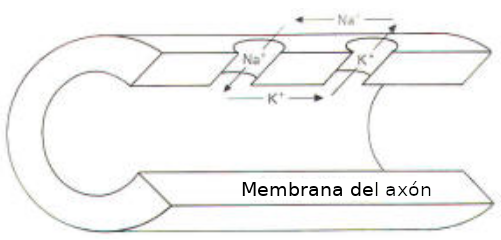
\includegraphics[width=7cm]{figures/corriente_membrana.png}
    \caption{Corriente a través de la membrana}
    \label{fig:corriente_membrana}
\end{figure}
\subsection{Resistencia y conductancia}\label{sec:resistencia_conductancia}
Todos los medios de conducción ofrecen algún grado de resistencia al paso de la corriente (indistintamente si es debido a la circulación de electrones o a la circulación de iones). La unidad de \textit{resistencia} R es el ohm ($\Omega$). El recíproco de la resistencia es la \textit{conductancia} g y su unidad es el siemens (S) aunque también se utiliza el término mho (ohm al revés) en la literatura clásica.
\begin{equation}
    \tcbhighmath[boxrule=1pt,arc=1pt,colback=blue!10!white,colframe=black]{g=\frac{1}{R}}
\end{equation}
Las membranas neuronales se comportan en parte como si estuvieran formadas por \textit{resistencias en paralelo} (fig.~\ref{fig:resistencia_fluidos}) mientras que los fluidos intracelulares y extracelulares que rodean a la membrana se comportan como \textit{resistencias en serie} (fig.~\ref{fig:resistencia_membrana}).
\begin{figure}[htbp!]
    \centering
    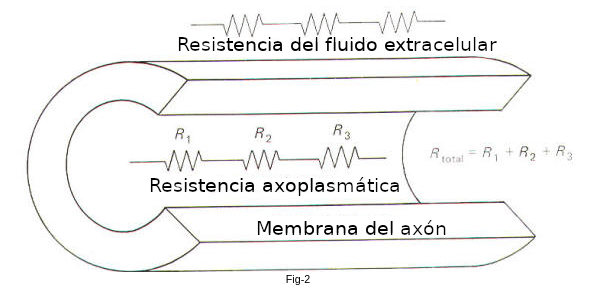
\includegraphics[width=9.0cm]{figures/Resistencia_Fluidos.png}
    \caption{Resistencia en serie del axoplasma y del fluido extracelular}
    \label{fig:resistencia_fluidos}
\end{figure}
La \textbf{\emph{resistencia de membrana}} representa la dificultad que tienen los iones en atravesarla a través sus respectivos canales. Su recíproco, \textbf{\emph{la conductancia}}, representa la facilidad que tienen los iones para atravesar la membrana.
\begin{figure}[htbp!]
            \centering 
            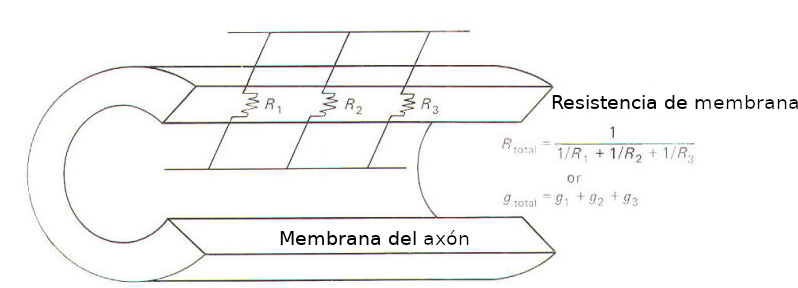
\includegraphics[width=11.0cm]{figures/Resistencia_Membrana.png}
            \caption{Membrana del axón en forma de resistencia en serie}
            \label{fig:resistencia_membrana}
\end{figure}

\subsection{Capacitancia}
 Un capacitor es un elemento que almacena energía en un campo eléctrico. Consiste en dos platos conductores separados por un dieléctrico y el mismo queda representado por un parámetro llamado \textit{capacitancia}:
\[C=\frac{\epsilon A}{d}\]
donde $\epsilon$ es la constante del dieléctrico, A es el área de los platos y d es la distancia que los separa. La unidad de la capacitancia es el \textit{faradio}.\\
La capacitancia es una medida de la habilidad que tiene un dispositivo para almacenar energía.\\
La carga almacenada por un capacitor es proporcional a su voltaje:
\[q= C.v\]
donde la constante de proporcionalidad C es la \textit{capacitancia} del capacitor.\\
La corriente se relaciona con la tensión mediante la ecuación diferencial:
\begin{equation}\label{eq:corriente_capacitor}
    \tcbhighmath[boxrule=1pt,arc=1pt,colback=blue!10!white,colframe=black]{i_c= C\dv{V}{t}}
\end{equation}
La membrana neuronal se comporta en parte como si estuviera compuesta por capacitores en paralelo (ver figura~\ref{fig:capacitores_paralelo_membrana}).
\begin{figure}[htbp!]
    \centering
    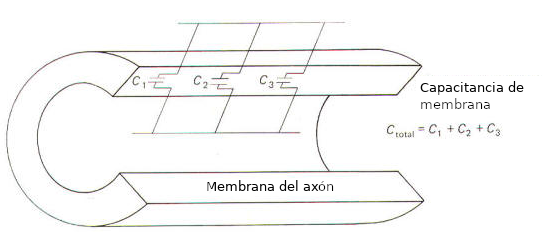
\includegraphics[width=9.0cm]{figures/capacitancia_membrana.png}
    \caption{Membrana como capacitores en paralelo}
    \label{fig:capacitores_paralelo_membrana}
\end{figure}
En la neurona, el interior de la membrana representa el dieléctrico, mientras que el fluido extracelular y el axoplasma representan los conductores (ver figura~\ref{fig:capacitor_membrana}).
\begin{figure}[htbp!]
    \centering
    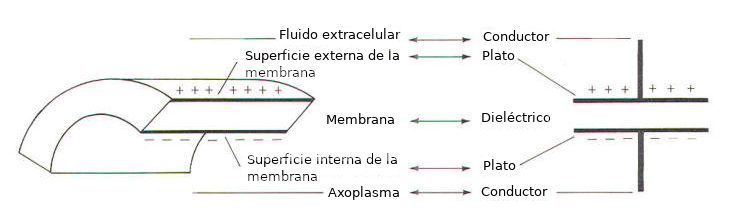
\includegraphics[width=11.5cm]{figures/dielectrico_neurona.png}
    \caption{Membrana como capacitor}
    \label{fig:capacitor_membrana}
\end{figure}
\textbf{\emph{La capacitancia de membrana representa la facilidad con que se carga la membrana}}
\subsection{Fuentes de tensión y de corriente}
La tensión eléctrica es la diferencia de potencial entre dos puntos. El voltaje a través de un elemento, es el trabajo (o la energía) requerido para mover una unidad de carga positiva desde la terminal negativa (-) hacia la terminal positiva (+). La unidad de voltaje es el volt (V). \cite{dorf2013introduction}.\\
Una fuente es un generador de tensión o de corriente, capaz de suministrar energía a un circuito. El generador de tensión es una fuente de carga (de electrones en circuitos eléctricos).\medskip \\ 
\textbf{\emph{En las neuronas, los iones representan la carga y el gradiente de concentración para un tipo de ion dado (ver~\ref{section:Potencial_Membrana}) representa la tensión de ese ion (el gradiente se puede representar mediante una fuente de tensión).}}\medskip \\
\textbf{\emph{La bomba sodio-potasio (ver~\ref{sec:bomba_sodio_potasio}) se puede representar mediante una fuente de corriente}}.
\begin{figure*}[htbp!]
        \centering
        \begin{subfigure}[b]{0.25\textwidth}
            \centering
            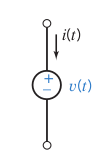
\includegraphics[width=2cm]{figures/fuente_tension.png}
            \caption{Fuente de tensión}
            \label{fig:fuente_tension}
        \end{subfigure}
       \hspace{0.5cm}
        \begin{subfigure}[b]{0.25\textwidth}  
            \centering 
            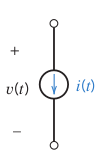
\includegraphics[width=2.0cm]{figures/fuente_corriente.png}
            \caption{Fuente de corriente}
            \label{fig:fuente_corriente}
        \end{subfigure}
        \quad
        \caption{Fuentes independientes}
        \label{fig:fuentes_independientes}
\end{figure*}
\section{Modelos eléctricos de entrada-salida}
La investigación más extensa realizada en esta categoría es la correspondiente al modelo de Hodking-Huxley \cite{HODGKIN1952}. En este modelo, el comportamiento eléctrico de la membrana puede ser representado por la red de la figura~\ref{fig:circuito_electrico_hodking_huxley}. 
\begin{figure}[htbp!]
    \centering
    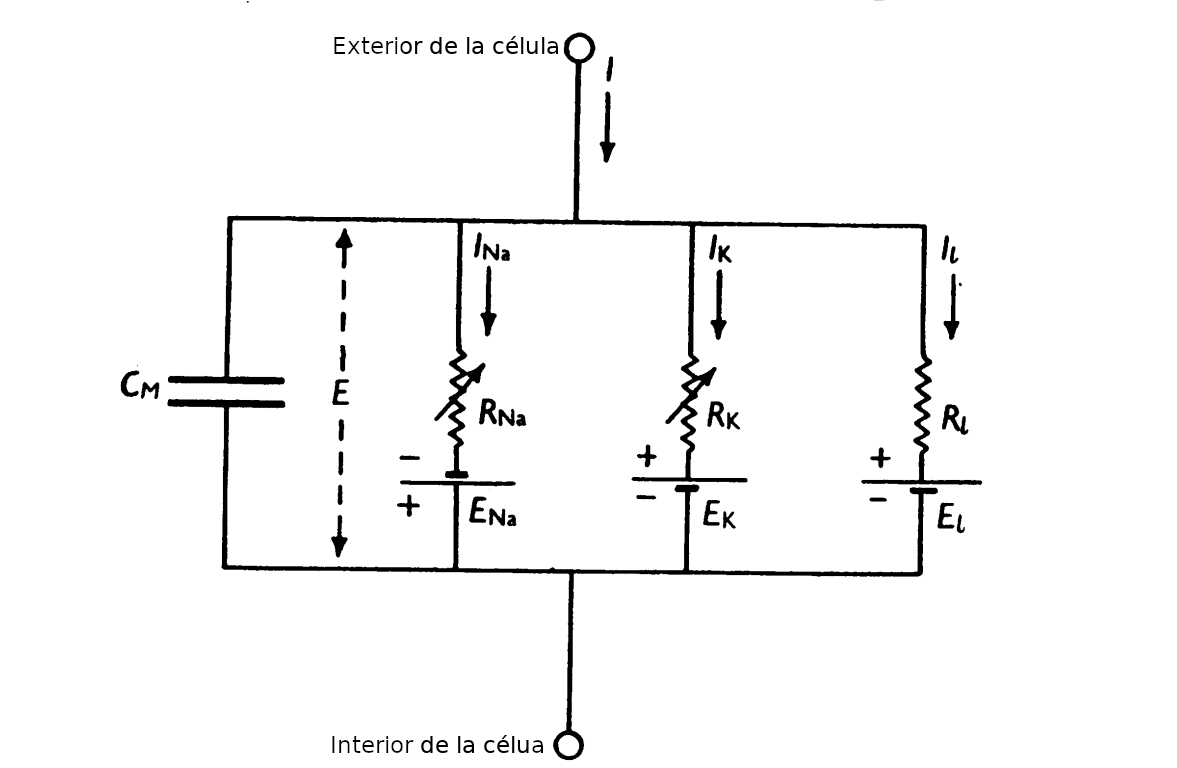
\includegraphics[width=10cm]{figures/Modelo_Hodking_Huxley+.png}
    \caption{Modelo de Hodgkin-Huxley. Circuto eléctrico que representa a una membrana. $R_{Na}=\frac{1}{g_{Na}}$, $R_{k}=\frac{1}{g_{k}}$, $R_{l}=\frac{1}{g_{l}}$. $R_{Na}$ y $R_k$ varían con el tiempo y el potencial de membrana. Los otros componentes son constantes}
    \label{fig:circuito_electrico_hodking_huxley}
\end{figure}
En el análisis realizado en \cite{HODGKIN1952}, se obtiene un conjunto de ecuaciones no lineales.
Existe una larga lista de modelos que derivan del modelo de Huxley-Hodgkin que tratan de simplificar la complejidad de las ecuaciones reduciendo el número de variables o los no linealidades asociadas. Uno de los objetivos es de reducir el cálculo computacional y permitir realizar simulaciones. En el presente trabajo se estudian modelos que derivan del \textit{integrate and fire}.
\subsection{Modelo Integrate and fire}
Es uno de los primeros modelos neuronales (1907). Se modela una neurona simplemente usando un capacitor (fig.~\ref{fig:integrate_and_fire}) y se plantea la ecuación~\ref{eq:corriente_capacitor} para determinar la corriente que circula por el mismo.
\begin{figure}[htbp!]
    \centering
    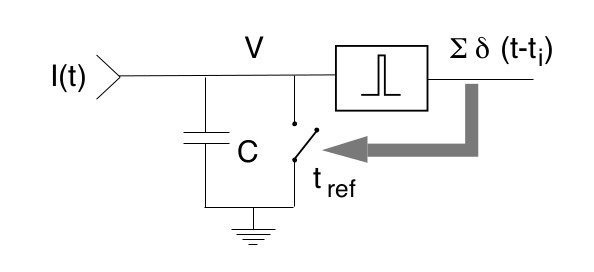
\includegraphics[width=10cm]{figures/prefect_integrate_and_fire.png}
    \caption{Integrate and fire}
    \label{fig:integrate_and_fire}
\end{figure}
Se caracteriza por tener un dominio de operación por debajo de un umbral y un voltaje umbral $v_{th}$ para la generación del impulso. El integrador perfecto, para lidiar con el modo de operación por debajo del umbral, utiliza simplemente un capacitor. Se asume que la corriente i(t) surge tanto desde una entrada sináptica como desde un electrodo intracelular.\\
La evolución del voltaje del integrador perfecto está gobernado por la ecuación diferencial de primer orden ~\ref{eq:corriente_capacitor}. Junto con la condición inicial, la ecuación~\ref{eq:corriente_capacitor} especifica la evolución en el tiempo del potencial de membrana durante la operación por debajo del umbral.\\
Una vez que el potencial llega a $v_th$, se dispara un impulso y el capacitor se conecta a tierra (cerrando la llave de la figura~\ref{fig:integrate_and_fire}) para descargar la carga que se había acumulado en el capacitor. Enviar la carga a tierra tiene el efecto instantáneo de resetear el potencial V(t) a cero. Se modela el potencial de acción asumiendo que en el instante t' en el cual $v(t')=v_{th}$, se genera un pulso de salida descrito por una función delta $\delta(t-t')$. Los tiempos sucesivos, $t_i$, de ocurrencia de un impulso se determinan recursivamente por la ecuación:
\[\int_{t_i}^{t_{i+1}} i(t) dt = C.v_{th}(t)\]
Una forma de caracterizar el comportamiento de la célula es mediante la relación entre la corriente inyectada y el promedio de la tasa de disparo (calculado como la inversa del intervalo entre impulsos).\\
En respuesta a una corriente aplicada en la entrada, el potencial de membrana va a cargar al capacitor hasta alcanzar $v_{th}$ y $v$ se resetea a 0 (cero). Cuanto mayor sea la corriente, menor va a ser el intervalo entre impulsos y más alta será el promedio de la tasa de disparo de acuerdo a:
\begin{equation}\label{eq:simple_firing_rate}
    <f>=\frac{i}{C.v_{th}}
\end{equation}
Hay unas cuestiones importantes que se desprenden de la ecuación~\ref{eq:simple_firing_rate}:
\begin{itemize}
    \item El promedio de la tasa de disparo depende linealmente de la corriente.
    \item Corrientes arbitrariamente pequeñas eventualmente van a producir un impulso, porque ninguna entrada se olvida. Cuando ingresa una corriente pequeña, esta corriente va a cargar al capacitor hasta una tensión determinada, menor a $v_{th}$. El capacitor va a mantener el valor de esa tensión (la va a recordar). A medida que ingresen más corrientes pequeñas que aporten una tensión menor a la umbral, estas tensiones se van a ir sumando hasta que en algún momento, la suma de todas ellas supere al umbral y produzca un disparo de un impulso.
    \item El tren de pulsos de salida es perfectamente regular. Las neuronas reales raramente, o nunca, responden a una corriente inyectada con un tren de pulsos espaciados de manera regular, sino que en realidad muestran una variabilidad en el tiempo entre impulsos (esto es lo que ocurre en el registro de neuronas \textit{in vivo}\cite{10.5555/1137840}).
\end{itemize}
El rango dinámico de la tasa de disparo de las células nerviosas está limitado por el hecho del que la corriente del sodio, responsable de la generación del impulso, se tiene que recuperar de la inactivación. Para simular el período refractario (sección~\ref{subsec:periodo_refractario}), hay que cerrar la llave de la figura~\ref{fig:integrate_and_fire} por un tiempo $t_{ref}$ determinado, poniendo en cero al potencial de membrana. Cualquier corriente que arribe durante ese tiempo va a ser desviada a tierra. Con esto se introduce una relación no lineal:
\begin{equation}
   \tcbhighmath[boxrule=1pt,arc=1pt,colback=blue!10!white,colframe=black]{ <f>=\frac{i}{C.v_{th}+t_{ref}.i}}
\end{equation}
La salida de este integrador frente a una entrada arbitraria de corriente consiste de una serie de impulsos $\sum_i \delta(t-t_i)$, todos espaciado al menos $t_{ref}$ entre sí. 
\newpage
\subsection{Modelo Leaky Integrate and fire}\label{sec:modelo_leaky_integrate_and_fire}
Para no tener la propiedad de \textit{memoria} y no recordar un valor de tensión no deseado, se agrega un término de fuga (\textit{leak}) al potencial de membrana. Este término refleja la difusión de iones cuando no se alcanza un estado de equilibrio en la célula.
\begin{figure}[htbp!]
    \centering
    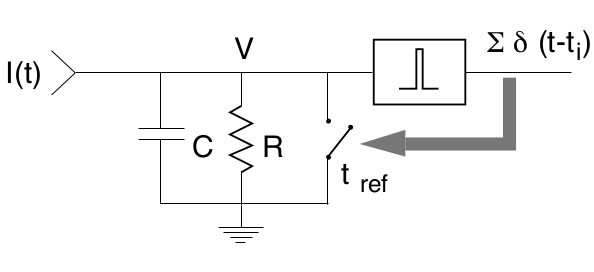
\includegraphics[width=10cm]{figures/leaky_integrate_and_fire.png}
    \caption{leaky Integrate and fire}
    \label{fig:leaky_integrate_and_fire}
\end{figure}
 El modelo \textit{leaky integrate and fire} tiene en cuenta esta fuga usando un circuito eléctrico formado por un capacitor y una resistencia en paralelo como se indica en la figura~\ref{fig:leaky_integrate_and_fire}.\\
Analizando la división de la corriente de entrada i(t), manteniendo la llave abierta (figura~\ref{fig:leaky_integrate_and_fire}), obtenemos:
\begin{equation}\label{eq:suma_corrientes_leaky}
    i(t)= i_R + i_C
\end{equation}
La corriente que atraviesa al capacitor ($i_c(t)$) es la que se indica en la ecuación~\ref{eq:corriente_capacitor}. La corriente que circula por la resistencia es:
\begin{equation}\label{eq:corriente_resistencia}
    \boxed{i_r(t)=\frac{v(t)}{R}}
\end{equation}
Reemplazando \ref{eq:corriente_capacitor} y \ref{eq:corriente_resistencia} en la ecuación~\ref{eq:corriente_resistencia},
\[
i(t)= C\dv{v}{t}+ \frac{v(t)}{R}
\]
Multiplicando por R:
\begin{equation}\label{eq:suma_corrientes_eq_diferencial_leaky}
    R.i(t)=RC \dv{v}{t} + v(t)
\end{equation}
La constante de tiempo del circuito es $\tau=RC$. Reemplazando RC por $\tau$ en la ecuación~\ref{eq:suma_corrientes_eq_diferencial_leaky}:
\begin{equation}\label{eq:ecuacion_diferencial_leaky}
    \tcbhighmath[boxrule=1pt,arc=1pt,colback=blue!10!white,colframe=black]{\tau \dv{v}{t} + v(t) = R.i(t)}
\end{equation}
\[\tcbhighmath[fuzzy halo=1mm with blue!50!white,arc=2pt,
  boxrule=0pt,frame hidden]{cond.\ inicial\ v(t=0)= 0}\]
\begin{center}
\begin{tabular}{ r l}
\footnotesize{donde,}&\\
 \footnotesize{$v(t)$:}& \footnotesize{es el potencial de membrana}\\ 
 \footnotesize{i(t)}:& \footnotesize{corriente de entrada.}\\
 \footnotesize{C:}& \footnotesize{capacitancia de membrana}\\
 \footnotesize{R}:& \footnotesize{resistencia de fuga (leak)}
\end{tabular}
\end{center}
En la versión general del modelo de neurona leaky integrate and fire se incorpora un \textit{período refractario} (ver secciones~\ref{subsec:fases_potencial_accion} y~\ref{subsec:periodo_refractario}):
\begin{enumerate}
    \item Si $v$ alcanza el valor umbral en un tiempo $t=T_{th}$, se interrumpe la dinámica de la ecuación~\ref{eq:ecuacion_diferencial_leaky} durante un tiempo refractario $t_{ref}$.
    \item Luego de un tiempo $T_{th}$+ $t_{ref}$ se reinicia la integración con la nueva condición inicial $v=0$.
\end{enumerate}
La ecuación~\ref{eq:ecuacion_diferencial_leaky} es una ecuación diferencial ordinaria\footnote{\textit{Ordinaria}: Se refiere a que la diferenciación se hace sólo con respecto a la variable independiente \textit{t}.}, de primer orden\footnote{\textit{Primer orden}: se refiere a que la derivada de orden mayor que se encuentra en la ecuación es la primera.}, lineal\footnote{\textit{Lineal} significa que la variable independiente y sus derivadas aparecen sólo como términos de primer grado, es decir, no hay términos del tipo $v^2(t)$ o $v(t).\dv{v}{t}$ (estos dos términos son de segundo grado).}, no homogénea\footnote{\footnotesize \textit{No homogénea}: significa que la ecuación incluye un término como g(t) donde g(t) puede ser una constante o alguna función conocida de t.} y de coeficientes constantes\footnote{\textit{Coeficientes constantes} significa que los coeficientes C y 1/R son constantes, es decir, no son funciones de la variable \textit{t}.}. Este sistema es un \textit{filtro pasabajos} (ver sección~\ref{sec:filtro_pasabajos_primer_orden}). \\
Si se aplica una corriente constante en forma de escalón (ver sección~\ref{sec:respuesta_escalon}), conectada en t=0 y permaneciendo igual de forma constante de ahí en adelante, la respuesta a esta entrada es la indicada en la ecuación~\ref{eq:respuesta_escalon_leaky_integrator}. En la misma se puede observar que la membrana se carga exponencialmente hasta su valor estacionario $v=i.R$. Sin embargo, el modelo integrate and fire sólo sigue esta ecuación siempre que el voltaje este por debajo la tensión umbral $v_{th}$. Una vez que se alcanza el umbral, se genera un impulso y la tensión se resetea a 0 (cero).\\
La corriente mínima necesaria para disparar un potencial de acción (corriente umbral) es:
\[i_{th}=\frac{v_{th}}{R}\]
Para cualquier corriente i mayor que $i_{th}$ se va a generar un pulso de salida en el instante $T_{th}$ tal que se mantenga el valor $v_{th}=i.R.\big(1-e^{-\frac{T_{th}}{\tau}}\big)$. Despejando $T_{th}$:
\[\frac{v_{th}}{i.R}=1-e^{-\frac{T_{th}}{\tau}}\]
\[\frac{v_{th}}{i.R}-1=-e^{-\frac{T_{th}}{\tau}}\]
\[1-\frac{v_{th}}{i.R}=e^{-\frac{T_{th}}{\tau}}\]
\[\ln{\Big(1-\frac{v_{th}}{i.R}\Big)}=-\frac{T_{th}}{\tau}\]
\begin{equation}
    \tcbhighmath[fuzzy halo=1mm with blue!50!white,arc=2pt,
  boxrule=0pt,frame hidden]{T_{th}=-\tau.\ln{\Big(1-\frac{v_{th}}{i.R}\Big)}}
\end{equation}
Como el voltaje se resetea después de un impulso y asumiendo que la corriente de entrada persiste, la membrana se va a cargar hasta el umbral, generando el siguiente impulso un tiempo $T_{th}+t_{ref}$ después. El promedio de la tasa de disparo es:
\begin{equation}
   \tcbhighmath[boxrule=1pt,arc=1pt,colback=blue!10!white,colframe=black]{ <f>=\frac{1}{t_{ref}+T_{th}}=\frac{1}{t_{ref}-\tau.\ln{\Big(1-\frac{v_{th}}{i.R}\Big)}}}
\end{equation}
